\section{Calculate Radar Plot Position}
\label{sec:calc_radar_pos}

Please note that if no Radar target reports exist in the database, this steps does not have to be performed.\\

Since in SASS-C Verif radar plot coordinates are not given as latitude/longitude, which are the main coordinates for all processing in ATSDB, optionally these coordinates can be re-calculated and set in the database using the ''Calculate Radar Plot Position`` Task. \\

To execute this task select 'Task'->  'Calculate Radar Plot Position' in the top menu bar. \\

Please note that for this step the data source positions have to set in the database, otherwise no plot position can be calculated. If a database generated by SASS-C is used, this should already be the case. For ones created by SDDL JSON, the steps described in \nameref{sec:data_source_editing} have to be performed once.

\begin{figure}[H]
  \center
    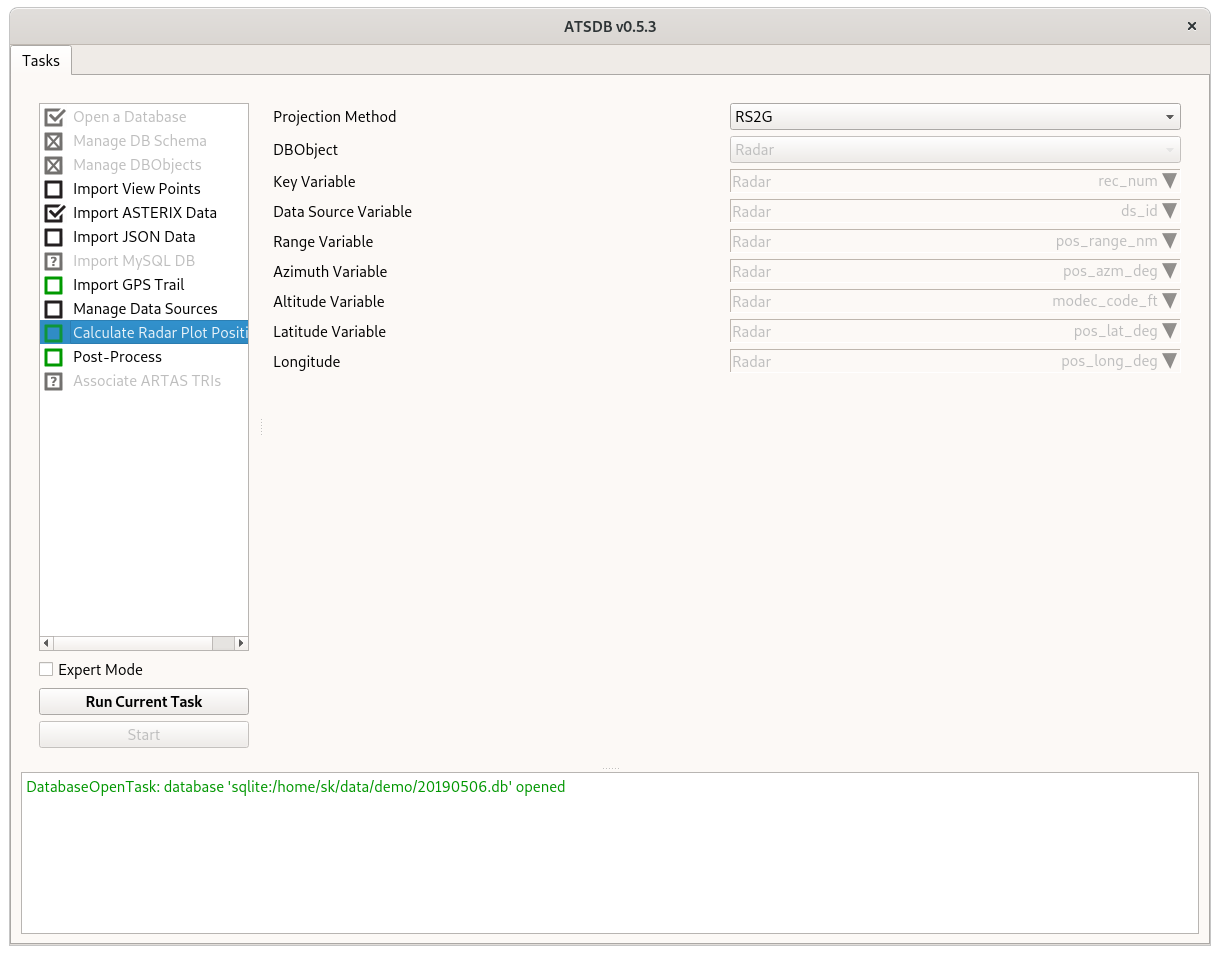
\includegraphics[width=14cm,frame]{../screenshots/task_calc_radar.png}
  \caption{Calculate radar plot position task}
  \label{fig:task_calc_radar}
\end{figure}

There are two projection methods (radar polar coordinates to WGS-84 coordinates) available. The \textit{RS2G} projection is the currently recommended option.

\paragraph{OGR Projection}

The EPSG code for the projection has to be chosen according to your needs, please refer to \url{http://spatialreference.org/ref/epsg/} for a list of possible codes.

The WGS84 latitude/longitude coordinates are then calculated using the radar positions in the database, the range and the azimuth. Please \textbf{note} that currently there will be offsets in the projected coordinates compared to the e.g. the ARTAS projection. The reason for this is under investigation.

\paragraph{RS2G Projection}

For this projection, no additional attributes must be given. Please \textbf{note} that this projection is based on a common 'radar slant to geodesic transformation', it should be equvalent to the ARTAS projection. A verification is still needed, please contact the author if you would be willing to support this.

\paragraph{Calculation}

Press 'Calculate' to start the calculation process, which will take a few minutes depending on the data size. \\

Messages like these will be printed in the text console, the last one indicates completion of the task:

The following windows will be shown, to give indication about the calculation progress:

\begin{figure}[H]
  \center
    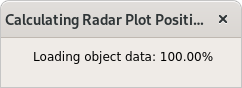
\includegraphics[width=4cm,frame]{../screenshots/task_calc_radar_load.png}
  \caption{Calculate radar plot position task: Loading}
\end{figure}

\begin{figure}[H]
  \center
    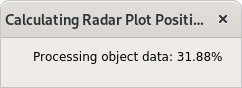
\includegraphics[width=4cm,frame]{../screenshots/task_calc_radar_process.png}
  \caption{Calculate radar plot position task: Processing}
\end{figure}

If there were projection errors in the calculation, the before insertion the user will be asked to confirm. The coordinates with projection errors will of course not be committed to the database, but will be skipped.

\begin{figure}[H]
  \center
    \includegraphics[width=9cm,frame]{../screenshots/task_calc_radar_insert.png}
  \caption{Calculate radar plot position task: Insertion question on errors}
\end{figure}


\begin{figure}[H]
  \center
    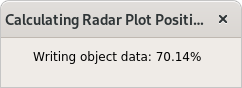
\includegraphics[width=4cm,frame]{../screenshots/task_calc_radar_write.png}
  \caption{Calculate radar plot position task: Writing}
\end{figure}

\begin{figure}[H]
  \center
    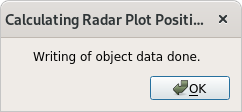
\includegraphics[width=8cm,frame]{../screenshots/task_calc_radar_done.png}
  \caption{Calculate radar plot position task: Done}
\end{figure}

After running this task once (per database), the radar plots also have a set latitude/longitude. As stated, a post-processing step is recommended after executing this task. \\

Please \textbf{note} that this task can be re-run with different projections if wanted.

Please \textbf{note} that no additional Radar plot information is changed, only the latitude/longitude variables are updated. 
